% last updated in April 2002 by Antje Endemann
% Based on CVPR 07 and LNCS, with modifications by DAF, AZ and elle, 2008 and AA, 2010, and CC, 2011; TT, 2014; AAS, 2016

\documentclass[runningheads]{llncs}
\usepackage{graphicx}
\usepackage{amsmath,amssymb} % define this before the line numbering.
\usepackage{ruler}
\usepackage{color}
\usepackage[width=122mm,left=12mm,paperwidth=146mm,height=193mm,top=12mm,paperheight=217mm]{geometry}
\begin{document}
% \renewcommand\thelinenumber{\color[rgb]{0.2,0.5,0.8}\normalfont\sffamily\scriptsize\arabic{linenumber}\color[rgb]{0,0,0}}
% \renewcommand\makeLineNumber {\hss\thelinenumber\ \hspace{6mm} \rlap{\hskip\textwidth\ \hspace{6.5mm}\thelinenumber}}
% \linenumbers
\pagestyle{headings}
\mainmatter
\def\ECCV18SubNumber{***}  % Insert your submission number here

\title{Author Guidelines for ECCV Submission} % Replace with your title

\titlerunning{ECCV-18 submission ID \ECCV18SubNumber}

\authorrunning{ECCV-18 submission ID \ECCV18SubNumber}

\author{Anonymous ECCV submission}
\institute{Paper ID \ECCV18SubNumber}


\maketitle

\begin{abstract}
The abstract should summarize the contents of the paper. LNCS guidelines
indicate it should be at least 70 and at most 150 words. It should be set in 9-point
font size and should be inset 1.0~cm from the right and left margins.
\dots
\keywords{We would like to encourage you to list your keywords within
the abstract section}
\end{abstract}


\section{Introduction}


This document serves as an example submission. It illustrates the format
we expect authors to follow when submitting a paper to ECCV. 
At the same time, it gives details on various aspects of paper submission,
including preservation of anonymity and how to deal with dual submissions,
so we advise authors to read this document carefully.

\section{Paper formatting}

\subsection{Language}

All manuscripts must be in English.

\subsection{Paper length}
Papers submitted for review should be complete. 
The length should match that intended for final publication. 
Papers accepted for the conference will be allocated 14 pages (plus references) in the proceedings. 
Note that the allocated 14 pages do not include the references. The reason for this policy
is that we do not want authors to omit references for sake of space limitations.

Papers with more than 14 pages (excluding references) will be rejected without review.
This includes papers where the margins and
formatting are deemed to have been significantly altered from those
laid down by this style guide.  The reason such papers will not be
reviewed is that there is no provision for supervised revisions of
manuscripts. The reviewing process cannot determine the suitability of
the paper for presentation in 14 pages if it is reviewed in 16.

\subsection{Paper ID}

It is imperative that the paper ID is mentioned on each page of the manuscript.
The paper ID is a number automatically assigned to your submission when 
registering your paper submission on CMT.


\subsection{Line numbering}

All lines should be numbered, as in this example document.  This makes
reviewing more efficient, because reviewers can refer to a line on a
page.  If you are preparing a document using a non-\LaTeX\
document preparation system, please arrange for an equivalent line numbering.



\subsection{Mathematics}

Please number all of your sections and displayed equations.  Again,
this makes reviewing more efficient, because reviewers can refer to a
line on a page.  Also, it is important for readers to be able to refer
to any particular equation.  Just because you didn't refer to it in
the text doesn't mean some future reader might not need to refer to
it.  It is cumbersome to have to use circumlocutions like ``the
equation second from the top of page 3 column 1''.  (Note that the
line numbering will not be present in the final copy, so is not an
alternative to equation numbers).  Some authors might benefit from
reading Mermin's description of how to write mathematics:
\url{www.pamitc.org/documents/mermin.pdf‎}.

\section{Blind review}
\label{sec:blind}

Many authors misunderstand the concept of anonymizing for blind
review.  Blind review does not mean that one must remove
citations to one's own work. In fact it is often impossible to
review a paper unless the previous citations are known and
available.

Blind review means that you do not use the words ``my'' or ``our''
when citing previous work.  That is all.  (But see below for
technical reports).

Saying ``this builds on the work of Lucy Smith [1]'' does not say
that you are Lucy Smith, it says that you are building on her
work.  If you are Smith and Jones, do not say ``as we show in
[7]'', say ``as Smith and Jones show in [7]'' and at the end of the
paper, include reference 7 as you would any other cited work.

An example of a bad paper:
\begin{quote}
\begin{center}
    An analysis of the frobnicatable foo filter.
\end{center}

   In this paper we present a performance analysis of our
   previous paper [1], and show it to be inferior to all
   previously known methods.  Why the previous paper was
   accepted without this analysis is beyond me.

   [1] Removed for blind review
\end{quote}


An example of an excellent paper:

\begin{quote}
\begin{center}
     An analysis of the frobnicatable foo filter.
\end{center}

   In this paper we present a performance analysis of the
   paper of Smith [1], and show it to be inferior to
   all previously known methods.  Why the previous paper
   was accepted without this analysis is beyond me.

   [1] Smith, L. and Jones, C. ``The frobnicatable foo
   filter, a fundamental contribution to human knowledge''.
   Nature 381(12), 1-213.
\end{quote}

If you are making a submission to another conference at the same
time, which covers similar or overlapping material, you may need
to refer to that submission in order to explain the differences,
just as you would if you had previously published related work. In
such cases, include the anonymized parallel
submission~\cite{Authors14} as additional material and cite it as
\begin{quote}
1. Authors. ``The frobnicatable foo filter'', BMVC 2014 Submission
ID 324, Supplied as additional material {\tt bmvc14.pdf}.
\end{quote}

Finally, you may feel you need to tell the reader that more
details can be found elsewhere, and refer them to a technical
report.  For conference submissions, the paper must stand on its
own, and not {\em require} the reviewer to go to a techreport for
further details.  Thus, you may say in the body of the paper
``further details may be found in~\cite{Authors14b}''.  Then
submit the techreport as additional material. Again, you may not
assume the reviewers will read this material.

Sometimes your paper is about a problem which you tested using a tool which
is widely known to be restricted to a single institution.  For example,
let's say it's 1969, you have solved a key problem on the Apollo lander,
and you believe that the ECCV audience would like to hear about your
solution.  The work is a development of your celebrated 1968 paper entitled
``Zero-g frobnication: How being the only people in the world with access to
the Apollo lander source code makes us a wow at parties'', by Zeus.

You can handle this paper like any other.  Don't write ``We show how to
improve our previous work [Anonymous, 1968].  This time we tested the
algorithm on a lunar lander [name of lander removed for blind review]''.
That would be silly, and would immediately identify the authors. Instead
write the following:
\begin{quotation}
\noindent
   We describe a system for zero-g frobnication.  This
   system is new because it handles the following cases:
   A, B.  Previous systems [Zeus et al. 1968] didn't
   handle case B properly.  Ours handles it by including
   a foo term in the bar integral.

   ...

   The proposed system was integrated with the Apollo
   lunar lander, and went all the way to the moon, don't
   you know.  It displayed the following behaviours
   which show how well we solved cases A and B: ...
\end{quotation}
As you can see, the above text follows standard scientific convention,
reads better than the first version, and does not explicitly name you as
the authors.  A reviewer might think it likely that the new paper was
written by Zeus, but cannot make any decision based on that guess.
He or she would have to be sure that no other authors could have been
contracted to solve problem B. \\

For sake of anonymity, it's recommended to omit acknowledgements
in your review copy. They can be added later when you prepare the final copy.



\section{Manuscript Preparation}

This is an edited version of Springer LNCS instructions adapted
for ECCV 2018 first paper submission.
You are strongly encouraged to use \LaTeX2$_\varepsilon$ for the
preparation of your
camera-ready manuscript together with the corresponding Springer
class file \verb+llncs.cls+.

We would like to stress that the class/style files and the template
should not be manipulated and that the guidelines regarding font sizes
and format should be adhered to. This is to ensure that the end product
is as homogeneous as possible.

\subsection{Printing Area}
The printing area is $122  \; \mbox{mm} \times 193 \;
\mbox{mm}$.
The text should be justified to occupy the full line width,
so that the right margin is not ragged, with words hyphenated as
appropriate. Please fill pages so that the length of the text
is no less than 180~mm.

\subsection{Layout, Typeface, Font Sizes, and Numbering}
Use 10-point type for the name(s) of the author(s) and 9-point type for
the address(es) and the abstract. For the main text, please use 10-point
type and single-line spacing.
We recommend using Computer Modern Roman (CM) fonts, Times, or one
of the similar typefaces widely used in photo-typesetting.
(In these typefaces the letters have serifs, i.e., short endstrokes at
the head and the foot of letters.)
Italic type may be used to emphasize words in running text. Bold
type and underlining should be avoided.
With these sizes, the interline distance should be set so that some 45
lines occur on a full-text page.

\subsubsection{Headings.}

Headings should be capitalized
(i.e., nouns, verbs, and all other words
except articles, prepositions, and conjunctions should be set with an
initial capital) and should,
with the exception of the title, be aligned to the left.
Words joined by a hyphen are subject to a special rule. If the first
word can stand alone, the second word should be capitalized.
The font sizes
are given in Table~\ref{table:headings}.
\setlength{\tabcolsep}{4pt}
\begin{table}
\begin{center}
\caption{Font sizes of headings. Table captions should always be
positioned {\it above} the tables. The final sentence of a table
caption should end without a full stop}
\label{table:headings}
\begin{tabular}{lll}
\hline\noalign{\smallskip}
Heading level & Example & Font size and style\\
\noalign{\smallskip}
\hline
\noalign{\smallskip}
Title (centered)  & {\Large \bf Lecture Notes \dots} & 14 point, bold\\
1st-level heading & {\large \bf 1 Introduction} & 12 point, bold\\
2nd-level heading & {\bf 2.1 Printing Area} & 10 point, bold\\
3rd-level heading & {\bf Headings.} Text follows \dots & 10 point, bold
\\
4th-level heading & {\it Remark.} Text follows \dots & 10 point,
italic\\
\hline
\end{tabular}
\end{center}
\end{table}
\setlength{\tabcolsep}{1.4pt}

Here are
some examples of headings: ``Criteria to Disprove Context-Freeness of
Collage Languages'', ``On Correcting the Intrusion of Tracing
Non-deterministic Programs by Software'', ``A User-Friendly and
Extendable Data Distribution System'', ``Multi-flip Networks:
Parallelizing GenSAT'', ``Self-determinations of Man''.

\subsubsection{Lemmas, Propositions, and Theorems.}

The numbers accorded to lemmas, propositions, and theorems etc. should
appear in consecutive order, starting with the number 1, and not, for
example, with the number 11.

\subsection{Figures and Photographs}
\label{sect:figures}

Please produce your figures electronically and integrate
them into your text file. For \LaTeX\ users we recommend using package
\verb+graphicx+ or the style files \verb+psfig+ or \verb+epsf+.

Check that in line drawings, lines are not
interrupted and have constant width. Grids and details within the
figures must be clearly readable and may not be written one on top of
the other. Line drawings should have a resolution of at least 800 dpi
(preferably 1200 dpi).
For digital halftones 300 dpi is usually sufficient.
The lettering in figures should have a height of 2~mm (10-point type).
Figures should be scaled up or down accordingly.
Please do not use any absolute coordinates in figures.

Figures should be numbered and should have a caption which should
always be positioned {\it under} the figures, in contrast to the caption
belonging to a table, which should always appear {\it above} the table.
Please center the captions between the margins and set them in
9-point type
(Fig.~\ref{fig:example} shows an example).
The distance between text and figure should be about 8~mm, the
distance between figure and caption about 5~mm.
\begin{figure}
\centering
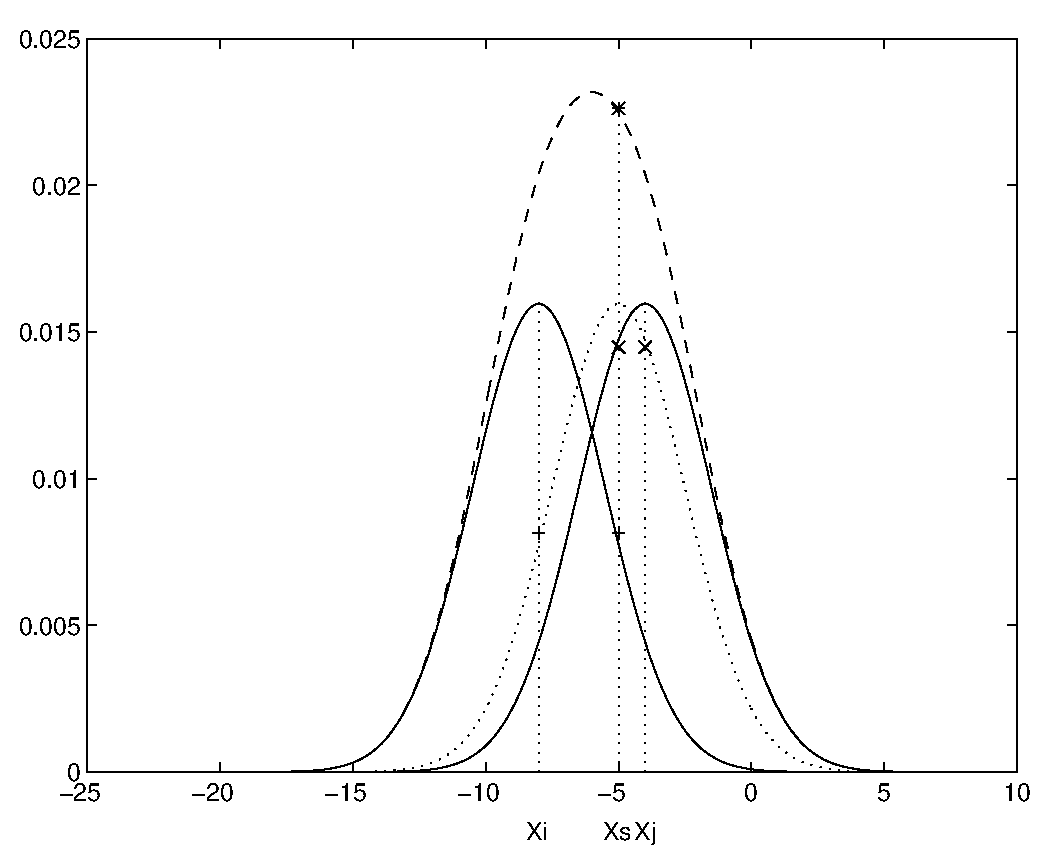
\includegraphics[height=6.5cm]{eijkel2}
\caption{One kernel at $x_s$ ({\it dotted kernel}) or two kernels at
$x_i$ and $x_j$ ({\it left and right}) lead to the same summed estimate
at $x_s$. This shows a figure consisting of different types of
lines. Elements of the figure described in the caption should be set in
italics,
in parentheses, as shown in this sample caption. The last
sentence of a figure caption should generally end without a full stop}
\label{fig:example}
\end{figure}

If possible (e.g. if you use \LaTeX) please define figures as floating
objects. \LaTeX\ users, please avoid using the location
parameter ``h'' for ``here''. If you have to insert a pagebreak before a
figure, please ensure that the previous page is completely filled.


\subsection{Formulas}

Displayed equations or formulas are centered and set on a separate
line (with an extra line or halfline space above and below). Displayed
expressions should be numbered for reference. The numbers should be
consecutive within the contribution,
with numbers enclosed in parentheses and set on the right margin.
For example,
\begin{align}
  \psi (u) & = \int_{0}^{T} \left[\frac{1}{2}
  \left(\Lambda_{0}^{-1} u,u\right) + N^{\ast} (-u)\right] dt \; \\
& = 0 ?
\end{align}

Please punctuate a displayed equation in the same way as ordinary
text but with a small space before the end punctuation.

\subsection{Footnotes}

The superscript numeral used to refer to a footnote appears in the text
either directly after the word to be discussed or, in relation to a
phrase or a sentence, following the punctuation sign (comma,
semicolon, or full stop). Footnotes should appear at the bottom of
the
normal text area, with a line of about 2~cm in \TeX\ and about 5~cm in
Word set
immediately above them.\footnote{The footnote numeral is set flush left
and the text follows with the usual word spacing. Second and subsequent
lines are indented. Footnotes should end with a full stop.}


\subsection{Program Code}

Program listings or program commands in the text are normally set in
typewriter font, e.g., CMTT10 or Courier.

\noindent
{\it Example of a Computer Program}
\begin{verbatim}
program Inflation (Output)
  {Assuming annual inflation rates of 7%, 8%, and 10%,...
   years};
   const
     MaxYears = 10;
   var
     Year: 0..MaxYears;
     Factor1, Factor2, Factor3: Real;
   begin
     Year := 0;
     Factor1 := 1.0; Factor2 := 1.0; Factor3 := 1.0;
     WriteLn('Year  7% 8% 10%'); WriteLn;
     repeat
       Year := Year + 1;
       Factor1 := Factor1 * 1.07;
       Factor2 := Factor2 * 1.08;
       Factor3 := Factor3 * 1.10;
       WriteLn(Year:5,Factor1:7:3,Factor2:7:3,Factor3:7:3)
     until Year = MaxYears
end.
\end{verbatim}
%
\noindent
{\small (Example from Jensen K., Wirth N. (1991) Pascal user manual and
report. Springer, New York)}



\subsection{Citations}

The list of references is headed ``References" and is not assigned a
number
in the decimal system of headings. The list should be set in small print
and placed at the end of your contribution, in front of the appendix,
if one exists.
Please do not insert a pagebreak before the list of references if the
page is not completely filled.
An example is given at the
end of this information sheet. For citations in the text please use
square brackets and consecutive numbers: \cite{Alpher02},
\cite{Alpher03}, \cite{Alpher04} \dots

\section{Conclusions}

The paper ends with a conclusion. 


\clearpage\mbox{}Page \thepage\ of the manuscript.
\clearpage\mbox{}Page \thepage\ of the manuscript.
\clearpage\mbox{}Page \thepage\ of the manuscript.
\clearpage\mbox{}Page \thepage\ of the manuscript.
\clearpage\mbox{}Page \thepage\ of the manuscript.
\clearpage\mbox{}Page \thepage\ of the manuscript.
\clearpage\mbox{}Page \thepage\ of the manuscript.
This is the last page of the manuscript.
\par\vfill\par
Now we have reached the maximum size of the ECCV 2018 submission (excluding references).
References should start immediately after the main text, but can continue on p.15 if needed.

\clearpage

\bibliographystyle{splncs}
\bibliography{egbib}
\end{document}
